\section*{Problem 1}
\subsection*{1A}
We start by looking for completely separable solutions, letting $y(x,t) = u(x)w(t)$, then
\begin{equation}
    \begin{split}
        \partial_{xx}y(x,t) &= \frac{1}{v^2}\partial_{tt}y(x,t)\\
        w(t)\partial_{xx}u(x) &= \frac{u(x)}{v^2}\partial_{tt}w(t)\\
        \frac{1}{u(x)}\partial_{xx}u(x) &= \frac{1}{v^2}\frac{1}{w(t)}\partial_{tt}w(t)
    \end{split}
\end{equation}
By construction, the left hand side does not depend on $t$ and the right hand side does not depend on $x$, so both sides must be equal to some constant $\mu$ independent of $x$ or $t$.
\begin{equation}
    \begin{split}
           \partial_{xx}u(x) &= \mu u(x)\\
           \partial_{tt}w(t) &= \mu v^2 w(t)
    \end{split}
\end{equation}
The general solution for $\mu = 0$ is
\begin{equation}
    \begin{split}
        u(x) &= A + Bx\\
        w(t) &= C + Dx
    \end{split}
\end{equation}
Applying the boundary conditions $u(0)=u(L)=0$
\begin{equation}
    \begin{split}
        u(0) &= A+B0=0\\
        u(L) &= BL = 0
    \end{split}
\end{equation}
So we can see that the only solution for $\mu=0$ are the trivial solutions. Assume then, without loss of generality, that $\mu \neq 0$, then we know that the general solution to a second order ODE is
\begin{equation}
    \begin{split}
        u(x) &= Ae^{\sqrt{\mu}x}+Be^{-\sqrt{\mu}x}\\
        w(t) &= Ce^{v\sqrt{\mu}t}+De^{-v\sqrt{\mu}t}
    \end{split}
\end{equation}
Applying the boundary conditions
\begin{equation}
    \begin{split}
        u(0) & = A + B = 0\\
        u(L) & = A(e^{\sqrt{\mu}L}-e^{-\sqrt{\mu}L}) = 0\\
        \implies e^{\sqrt{\mu}L}&=e^{-\sqrt{\mu}L}\\
        e^{2\sqrt{\mu}L} &= 1\\
        \implies 2\sqrt{\mu}L &= i2\pi k\\
        \sqrt{\mu} &= \frac{i\pi k}{L}
    \end{split}
\end{equation}
Where $k \in \mathbb{Z}/\{0\}$ ($k=0$ represents the trivial solution). We can substitute $u(x)$ and $w(t)$ using complex-trig identities and elbow grease to obtain
\begin{equation}
    \begin{split}
        u_k(x) &= 2iA\sin(\frac{\pi k}{L}x)\\
        w_k(t) &= 2(C+D)\cos(v\frac{\pi k}{L}t)+i(C-D)\sin(v\frac{\pi k}{L}t)\\
    \end{split}
\end{equation}
Since our original PDE is linear any combination of $u_kw_k$ is also a solution, so the general solution is
\begin{equation}
    \psi(x,t) = \sum_k\sin(\frac{\pi k}{L}x)(A_k\cos(v\frac{\pi k}{L}t)+B_k\sin(v\frac{\pi k}{L}t))
\end{equation}
Where the coefficients $A_k = i4(C+D)$ and $B_k = -2(C-D)$.

We then assume our system has been "prepared" in a particular state. That is, at $t=0$, our system is unchanging $\psi'(x,0)=0$.
\begin{equation}
\begin{split}
        \psi'(x,0) &= \sum_k\sin(\frac{k\pi}{L}x)\frac{vk\pi}{L}\beta_k=0\\
        \implies \beta_k &= 0\\
        \implies \psi(x,t) &=  \sum_kA_k\sin(\frac{\pi k}{L}x)\cos(v\frac{\pi k}{L}t)
\end{split}
\end{equation}
The coefficients $A_j$ depend on $\psi(x,0)$ as follows
\begin{equation}
\begin{split}
    \psi(x,0) &= \sum_k\sin(\frac{\pi k}{L}x)A_k\\
    A_j &= \frac{2}{L}\int_0^Ldx\psi(x,0)\sin(\frac{\pi j}{L}x)
\end{split}
\end{equation}

\subsection*{1B}
The initial conditions are
\begin{equation}
    y(x,0) = \begin{cases}
        \frac{2dx}{L} &0 \leq x \leq \frac{L}{2}\\
        \frac{2d(L-x)}{L} & \frac{L}{2} \leq x \leq L
    \end{cases}
\end{equation}
The coefficients are
\begin{equation}
    \begin{split}
        A_j &= \frac{2}{L}\int_0^{\frac{L}{2}}dx\frac{2dx}{L}\sin(\frac{\pi j}{L}x)+\frac{2}{L}\int_{\frac{L}{2}}^Ldx\frac{2d(L-x)}{L}\sin(\frac{\pi j}{L}x)\\
        &=\sin(\frac{\pi}{2}j)\frac{8d}{\pi^2j^2}\\
        A_1 &= \frac{8d}{\pi^2}\\
        A_2 &= \frac{8d}{\pi^24}\\
        A_3 &= -\frac{8d}{\pi^29}
    \end{split}
\end{equation}
Letting $v=0.5$, the wave evolution is plotted below
\begin{figure}[h]
    \centering
    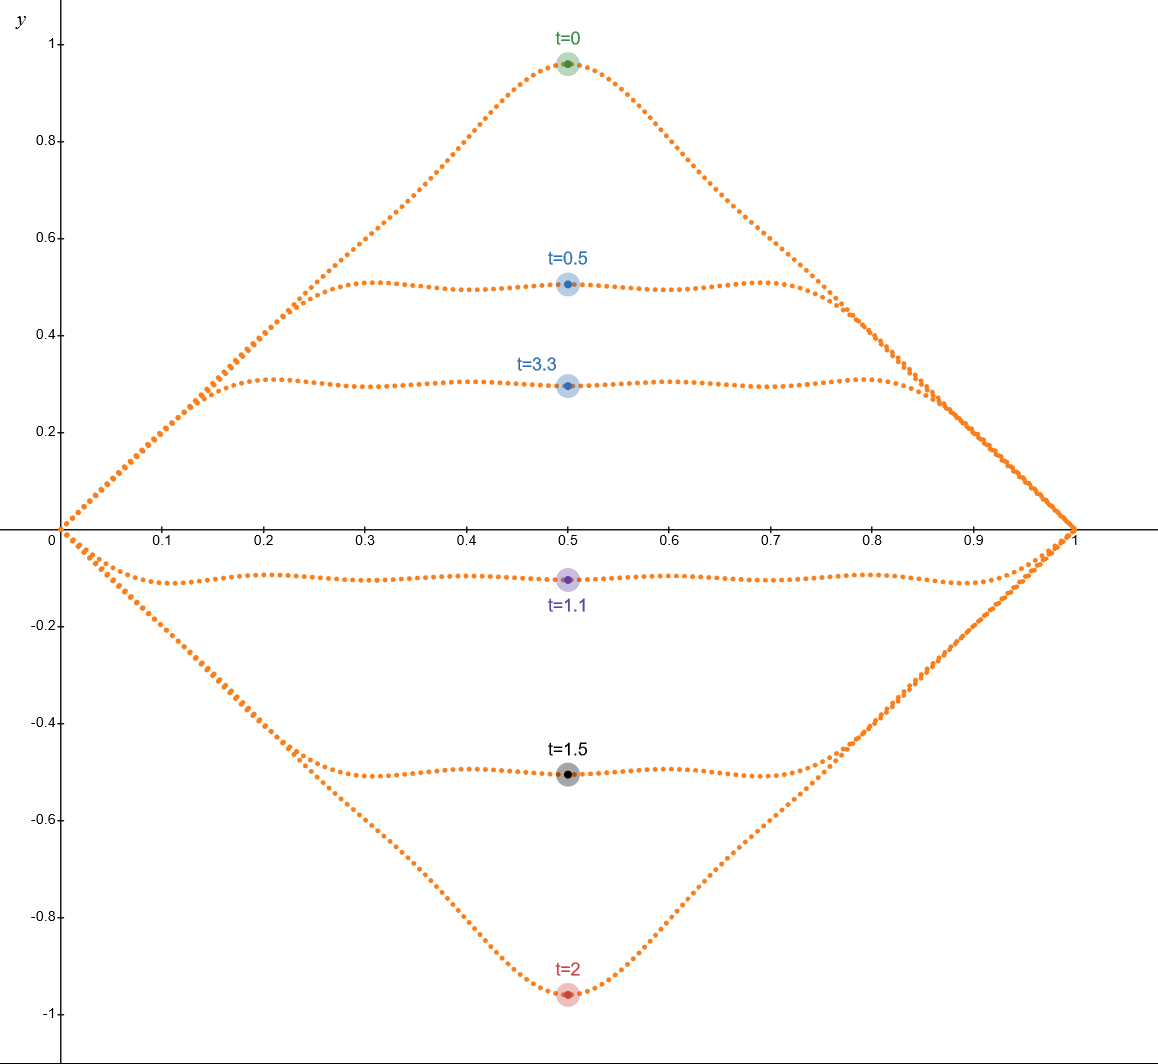
\includegraphics[width=0.5\linewidth]{Resources/245/245 Homework 1 Problem 1.png}
    \caption{$6$ terms are plotted in time}
    \label{fig:initial}
\end{figure}

\subsection*{1C}
Here we make two observations, the completely separable solutions form an orthogonal basis for a subspace of the vector space of solutions; which is why $\beta_k = 0$ for all $k$. This basis is sufficient for approximating "nearly" any function in $L^2$ so we're guaranteed that "nearly" all of our solutions (at least in $\L^2$) are represented by some linear combination of our completely separable solutions.

\pagebreak
\section*{Problem 2}
The figure below contains plots of the magnitude of $a_1(t)$ and $a_2(t)$ for both the original ODE (green) and the RWA (red).

\begin{figure}[h]
    \centering
    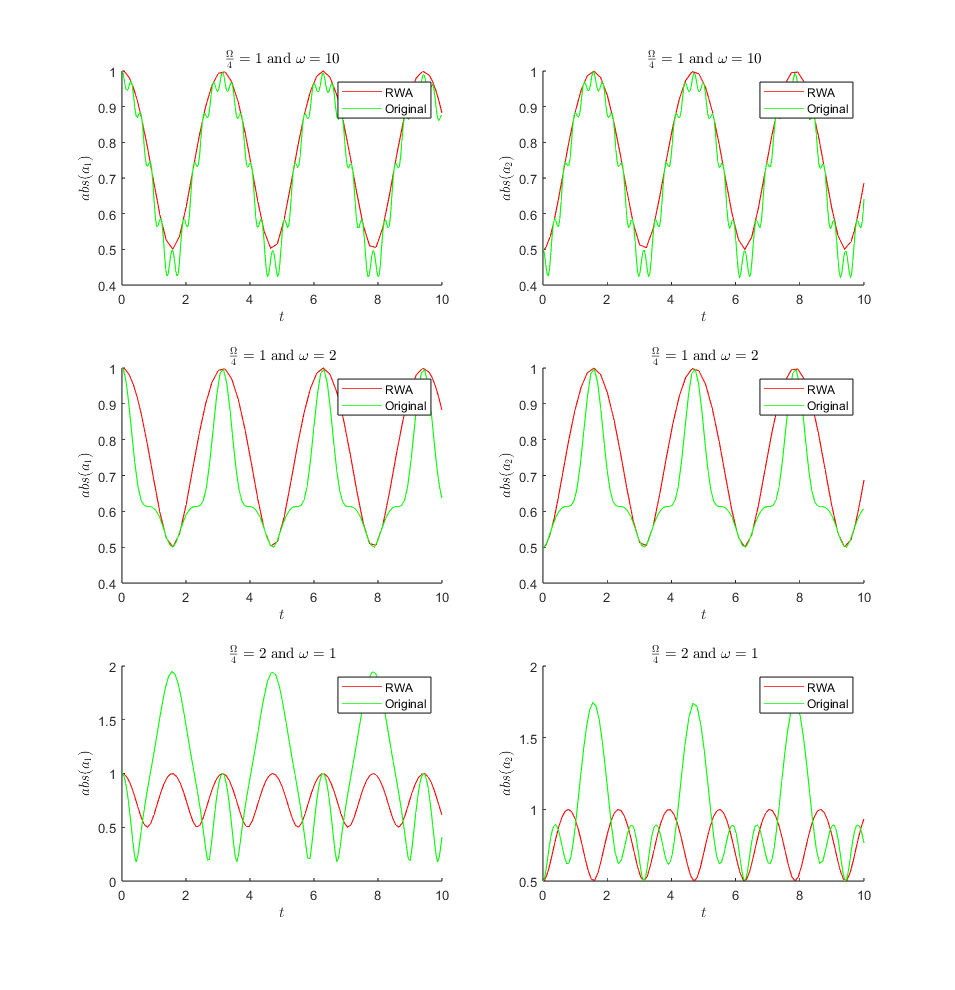
\includegraphics[width=1\linewidth]{Resources//245/245 Homework 1 Problem 2.png}
    \caption{RWA approximation for $\frac{\Omega}{4}=1,1,2$ and $\omega=10,2,1$.}
    \label{fig:rwa}
\end{figure}


\section*{Problem 3}

\subsection*{3A}

\begin{equation}
    \begin{split}
        e^{Mt} &= \sum_{n=0}^\infty \frac{1}{n!}(Mt)^n\\
        &=\sum_{n=0}^\infty\frac{1}{n!}(-lt\frac{\Omega}{4\hbar})^n\sigma_x^n\\
        &=I_2-(lt\frac{\Omega}{4\hbar})\sigma_x+\frac{1}{2!}(lt\frac{\Omega}{4\hbar})^2I_2-\frac{1}{3!}(lt\frac{\Omega}{4\hbar})^3\sigma_x+\dots
    \end{split}
\end{equation}

Then
\begin{equation}
    \begin{split}
        \vec{a}_{11} = \vec{a}_{22} &= 1+\frac{1}{2!}(lt\frac{\Omega}{4\hbar})^2+\frac{1}{4!}(lt\frac{\Omega}{4\hbar})^4 + \dots\\
        \vec{a}_{12} = \vec{a}_{21} &= -(lt\frac{\Omega}{4\hbar})-\frac{1}{3!}(lt\frac{\Omega}{4\hbar})^3-\frac{1}{5!}(lt\frac{\Omega}{4\hbar})^5-\dots
    \end{split}
\end{equation}
So
\begin{equation}
    e^{Mt} =
    \begin{pmatrix}
    \cosh(l\frac{\Omega}{4\hbar}t) & -\sinh(l\frac{\Omega}{4\hbar}t) \\
    -\sinh(l\frac{\Omega}{4\hbar}t) & \cosh(l\frac{\Omega}{4\hbar}t)\\
    \end{pmatrix}
\end{equation}
So the solution to our IVP is
\begin{equation}
    \vec{a}(t) =     \begin{pmatrix}
    \cosh(l\frac{\Omega}{4\hbar}t) & -\sinh(l\frac{\Omega}{4\hbar}t) \\
    -\sinh(l\frac{\Omega}{4\hbar}t) & \cosh(l\frac{\Omega}{4\hbar}t)\\
    \end{pmatrix} a_0
\end{equation}
\newpage
\subsection*{3B}
\begin{figure}[h]
    \centering
    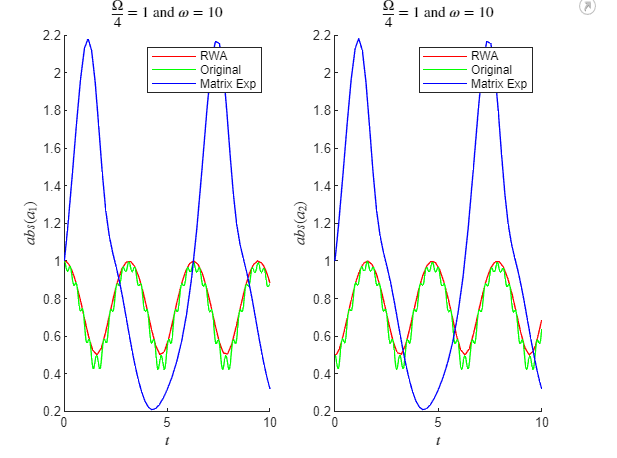
\includegraphics[width=0.75\linewidth]{Resources//245/245 Homework 1 Problem 3b.png}
    \caption{Comparison of matrix exponential to RWA and original DE using parameters from 2a}
    \label{fig:enter-label}
\end{figure}

\section*{Problem 4}

\subsection*{4A}
The Schrodinger equation for a particle in an infinite square well of width $L$ is
\begin{equation}
    \begin{split}
        -\frac{\hbar^2}{2m}\partial_{xx}\psi = E\psi
    \end{split}
\end{equation}
The general solution is
\begin{equation}
    \psi(x)=Ae^{-i\frac{\sqrt{pmE}}{\hbar}}+Be^{i\frac{\sqrt{pmE}}{\hbar}}
\end{equation}
Applying the boundary conditions, exactly as in problem 1, the normalized solutions are
\begin{equation}
    \psi_k(x)=\sqrt{\frac{2}{L}}\sin(\frac{\pi k}{L}x)
\end{equation}
The expectation values of position and momentum are
\begin{equation}
    \begin{split}
        \braket{\hat{x}} &= \frac{2}{L}\int_0^Lx\sin^2(\frac{\pi k}{L}x)=\frac{L}{2}\\
        \braket{\hat{p}} &= \frac{2}{L}\int_0^L\sin(\frac{\pi k}{L}x)(-i\hbar\partial_x)\sin(\frac{\pi k}{L}x) = 0
    \end{split}
\end{equation}

\subsection*{4B}
\begin{equation}
    \begin{split}
        \braket{\hat{x}^2} &= \frac{2}{L}\int_0^Lx^2\sin^2(\frac{\pi k}{L}x)=L^2(\frac{1}{3}-\frac{1}{2k^2\pi^2})\\
        \braket{\hat{p}^2} &= \frac{2}{L}\int_0^L\sin(\frac{\pi k}{L}x)(-i\hbar\partial_x)^2\sin(\frac{\pi k}{L}x) = (\frac{\hbar \pi k}{L})^2
    \end{split}
\end{equation}
The uncertainty is then
\begin{equation}
    \begin{split}
        \sigma_x&=\sqrt{\braket{\hat{x}^2}-\braket{\hat{x}}^2}=L\sqrt{\frac{1}{12}-\frac{1}{2k^2\pi^2}}\\
        \sigma_p &= \sqrt{\braket{\hat{p}^2}-\braket{\hat{p}}^2} = \frac{\hbar \pi k}{L}
    \end{split}
\end{equation}

\section*{Problem 5}

\subsection*{5A}
The expectation values are
\begin{equation}
    \begin{split}
        \braket{\hat{S}^2} &= \braket{\uparrow|\hat{S}^2|\uparrow} = \frac{3}{4}\hbar^2 \braket{\uparrow|\uparrow} = \frac{3}{4}\hbar^2\\
        \braket{(\hat{S}^2)^2} &= \braket{\uparrow|(\hat{S}^2)^2|\uparrow} = (\frac{3}{4}\hbar^2)^2 \braket{\uparrow|\uparrow} = (\frac{3}{4}\hbar^2)^2\\
        \braket{\hat{S_x}} &= \braket{\uparrow | \hat{S}_x|\uparrow} = \frac{\hbar}{2}\begin{pmatrix}
            1 & 0
        \end{pmatrix}
        \begin{pmatrix}
            0 & 1\\
            1 & 0
        \end{pmatrix}
        \begin{pmatrix}
            1\\0
        \end{pmatrix} = 0\\
        \braket{\hat{S_z}} &= \braket{\uparrow | \hat{S}_z|\uparrow} = \frac{\hbar}{2}\begin{pmatrix}
            1 & 0
        \end{pmatrix}
        \begin{pmatrix}
            1 & 0\\
            0 & -1
        \end{pmatrix}
        \begin{pmatrix}
            1\\0
        \end{pmatrix} = \frac{\hbar}{2}\\
        \braket{\hat{S}_x^2} &= \braket{\hat{S}_z^2} = (\frac{\hbar}{2})^2\braket{\uparrow|I_2|\uparrow} = (\frac{\hbar}{2})^2
    \end{split}
\end{equation}
The uncertainty is then
\begin{equation}
    \begin{split}
        \sigma_{\hat{S}^2} &= \sqrt{(\frac{3}{4}\hbar^2)^2-(\frac{3}{4}\hbar^2)^2}=0\\
        \sigma_{\hat{S}_x} &= \sqrt{(\frac{\hbar}{2})^2-0^2}=\frac{\hbar}{2}\\
        \sigma_{\hat{S}_z} &= \sqrt{(\frac{\hbar}{2})^2-(\frac{\hbar}{2})^2} = 0
    \end{split}
\end{equation}

\subsection*{5B}
The expectation values are
\begin{equation}
    \begin{split}
        \braket{\hat{S}^2} 
        &= \frac{1}{2}(\bra{\uparrow}+\bra{\downarrow})(\hat{S}^2\ket{\uparrow}+\hat{S}^2\ket{\downarrow}) \\
        &= \frac{1}{2}\frac{3}{4}\hbar(\bra{\uparrow}+\bra{\downarrow})(\ket{\uparrow}+\ket{\downarrow}) = \frac{3}{4}\hbar\\
        \braket{(\hat{S}^2)^2}
        &= \frac{1}{2}(\bra{\uparrow}+\bra{\downarrow})((\hat{S}^2)^2\ket{\uparrow}+(\hat{S}^2)^2\ket{\downarrow})\\
        &= \frac{1}{2}(\frac{3}{4}\hbar)^2(\bra{\uparrow}+\bra{\downarrow})(\ket{\uparrow}+\ket{\downarrow}) = (\frac{3}{4}\hbar)^2\\
        \braket{\hat{S}_x} 
        &= \frac{1}{2}(\bra{\uparrow}+\bra{\downarrow})(\hat{S}_x\ket{\uparrow}+\hat{S}_x\ket{\downarrow})\\
        &=\frac{1}{2}\frac{\hbar}{2}
        \begin{pmatrix}
            1 & 1
        \end{pmatrix}
        \begin{pmatrix}
            0 & 1\\
            1 & 0
        \end{pmatrix}
        \begin{pmatrix}
            1\\1
        \end{pmatrix} = \frac{\hbar}{2}\\
        \braket{\hat{S}_z}
        &= \frac{1}{2}(\bra{\uparrow}+\bra{\downarrow})(\hat{S}_z\ket{\uparrow}+\hat{S}_z\ket{\downarrow})\\
        &=\frac{1}{2}\frac{\hbar}{2}
        \begin{pmatrix}
            1 & 1
        \end{pmatrix}
        \begin{pmatrix}
            1 & 0\\
            0 & -1
        \end{pmatrix}
        \begin{pmatrix}
            1\\1
        \end{pmatrix} = 0\\
        \braket{\hat{S}_x^2}
        &= \braket{\hat{S}_z^2} = \frac{1}{2}(\bra{\uparrow}+\bra{\downarrow})(\hat{S}_x^2\ket{\uparrow}+\hat{S}_x^2\ket{\downarrow})\\
        &= \frac{1}{2}(\frac{\hbar}{2})^2(\bra{\uparrow}+\bra{\downarrow})(I_2\ket{\uparrow}+I_2\ket{\downarrow}) = (\frac{\hbar}{2})^2
    \end{split}
\end{equation}
The uncertainty is then
\begin{equation}
    \begin{split}
        \sigma_{\hat{S}^2} &= \sqrt{(\frac{3}{4}\hbar)^2-(\frac{3}{4}\hbar)^2} = 0\\
        \sigma_{\hat{S}_x} &= \sqrt{(\frac{\hbar}{2})^2-(\frac{\hbar}{2})^2} = 0\\
        \sigma_{\hat{S}_z} &= \sqrt{(\frac{\hbar}{2})^2-0^2}=\frac{\hbar}{2}
    \end{split}
\end{equation}